\documentclass[11pt, a4paper]{article}
\usepackage{pdfpages}
\usepackage{parallel}
\usepackage[T2A]{fontenc}
\usepackage{ucs}
\usepackage[utf8x]{inputenc}
\usepackage[polish,english,russian]{babel}
\usepackage{hyperref}
\usepackage{rotating}
\usepackage[inner=2cm,top=1.8cm,outer=2cm,bottom=2.3cm,nohead]{geometry}
\usepackage{listings}
\usepackage{graphicx}
\usepackage{wrapfig}
\usepackage{longtable}
\usepackage{indentfirst}
\usepackage{array}
\usepackage{tikzsymbols}
\usepackage{soul}
\usepackage[ruled,vlined]{algorithm2e}
%\counterwithout{figure}{section} 

\usepackage{url}
\makeatletter
\g@addto@macro{\UrlBreaks}{\UrlOrds}
\makeatother

\newcolumntype{P}[1]{>{\raggedright\arraybackslash}p{#1}}
\frenchspacing
\usepackage{fixltx2e} %text sub- and superscripts
\usepackage{icomma} % коскі ў матэматычным рэжыме
\PreloadUnicodePage{4}

\newcommand{\longpage}{\enlargethispage{\baselineskip}}
\newcommand{\shortpage}{\enlargethispage{-\baselineskip}}

\def\switchlang#1{\expandafter\csname switchlang#1\endcsname}
\def\switchlangbe{
\let\saverefname=\refname%
\def\refname{Літаратура}%
\def\figurename{Іл.}%
}
\def\switchlangen{
\let\saverefname=\refname%
\def\refname{References}%
\def\figurename{Fig.}%
}
\def\switchlangru{
\let\saverefname=\refname%
\let\savefigurename=\figurename%
\def\refname{Литература}%
\def\figurename{Рис.}%
}

\hyphenation{admi-ni-stra-tive}
\hyphenation{ex-pe-ri-ence}
\hyphenation{fle-xi-bi-li-ty}
\hyphenation{Py-thon}
\hyphenation{ma-the-ma-ti-cal}
\hyphenation{re-ported}
\hyphenation{imp-le-menta-tions}
\hyphenation{pro-vides}
\hyphenation{en-gi-neering}
\hyphenation{com-pa-ti-bi-li-ty}
\hyphenation{im-pos-sible}
\hyphenation{desk-top}
\hyphenation{elec-tro-nic}
\hyphenation{com-pa-ny}
\hyphenation{de-ve-lop-ment}
\hyphenation{de-ve-loping}
\hyphenation{de-ve-lop}
\hyphenation{da-ta-ba-se}
\hyphenation{plat-forms}
\hyphenation{or-ga-ni-za-tion}
\hyphenation{pro-gramming}
\hyphenation{in-stru-ments}
\hyphenation{Li-nux}
\hyphenation{sour-ce}
\hyphenation{en-vi-ron-ment}
\hyphenation{Te-le-pathy}
\hyphenation{Li-nux-ov-ka}
\hyphenation{Open-BSD}
\hyphenation{Free-BSD}
\hyphenation{men-ti-on-ed}
\hyphenation{app-li-ca-tion}

\def\progref!#1!{\texttt{#1}}
\renewcommand{\arraystretch}{2} %Іначай формулы ў матрыцы зліпаюцца з лініямі
\usepackage{array}

\def\interview #1 (#2), #3, #4, #5\par{

\section[#1, #3, #4]{#1 -- #3, #4}
\def\qname{LVEE}
\def\aname{#1}
\def\q ##1\par{{\noindent \bf \qname: ##1 }\par}
\def\a{{\noindent \bf \aname: } \def\qname{L}\def\aname{#2}}
}

\def\interview* #1 (#2), #3, #4, #5\par{

\section*{#1\\{\small\rm #3, #4. #5}}
\ifx\ParallelWhichBox\undefined%
    \addcontentsline{toc}{section}{#1, #3, #4}%
\else%
\ifnum\ParallelWhichBox=0%
    \addcontentsline{toc}{section}{#1, #3, #4}%
\fi\fi%

\def\qname{LVEE}
\def\aname{#1}
\def\q ##1\par{{\noindent \bf \qname: ##1 }\par}
\def\a{{\noindent \bf \aname: } \def\qname{L}\def\aname{#2}}
}

\newcommand{\interviewfooter}[1]{
\vskip 1em
\noindent \textit{#1}
}


\begin{document}

\title{1995 "--- ProAgio Scroll Mouse}
\date{}
\maketitle

В настоящий момент колесо прокрутки является настолько неотъемлемой частью работы с мышью, что трудно представить себе использование графического интерфейса без него.

    Первая серийно выпускавшаяся мышь с колесом прокрутки, - это мышь Genius EasyScroll, выпущенная в 1995 году, известная также как ProAgio Scroll Mouse.
    
    Мышь имеет эргномичную форму, также перекликающуюся с формой Microsoft Dove Bar mouse, но в отличие от мыши Prohance, устройство оснащено пятью кнопками, которые имеют достаточно большую площадь и ребристые края, удобно ложатся в руку, а левая кнопка снабжена рельефной поверхностью для более легкой тактильной идентификации. Колесо прокрутки расположено посередине корпуса в его передней части, и оно намного шире, чем в более поздних версиях (фактически, это можно было бы назвать роликом или барабаном). Помимо функции колеса прокрутки, оно реагирует на нажатие как на кнопку, как в большинстве современных мышей. Также пользователю доступна вытянутая узкая кнопка на боковой стороен корпуса для нажатия большим палцем. Предположительно, функции кнопок можно переназначать с помощью программного обеспечения.

\begin{figure}[h]
        \centering
    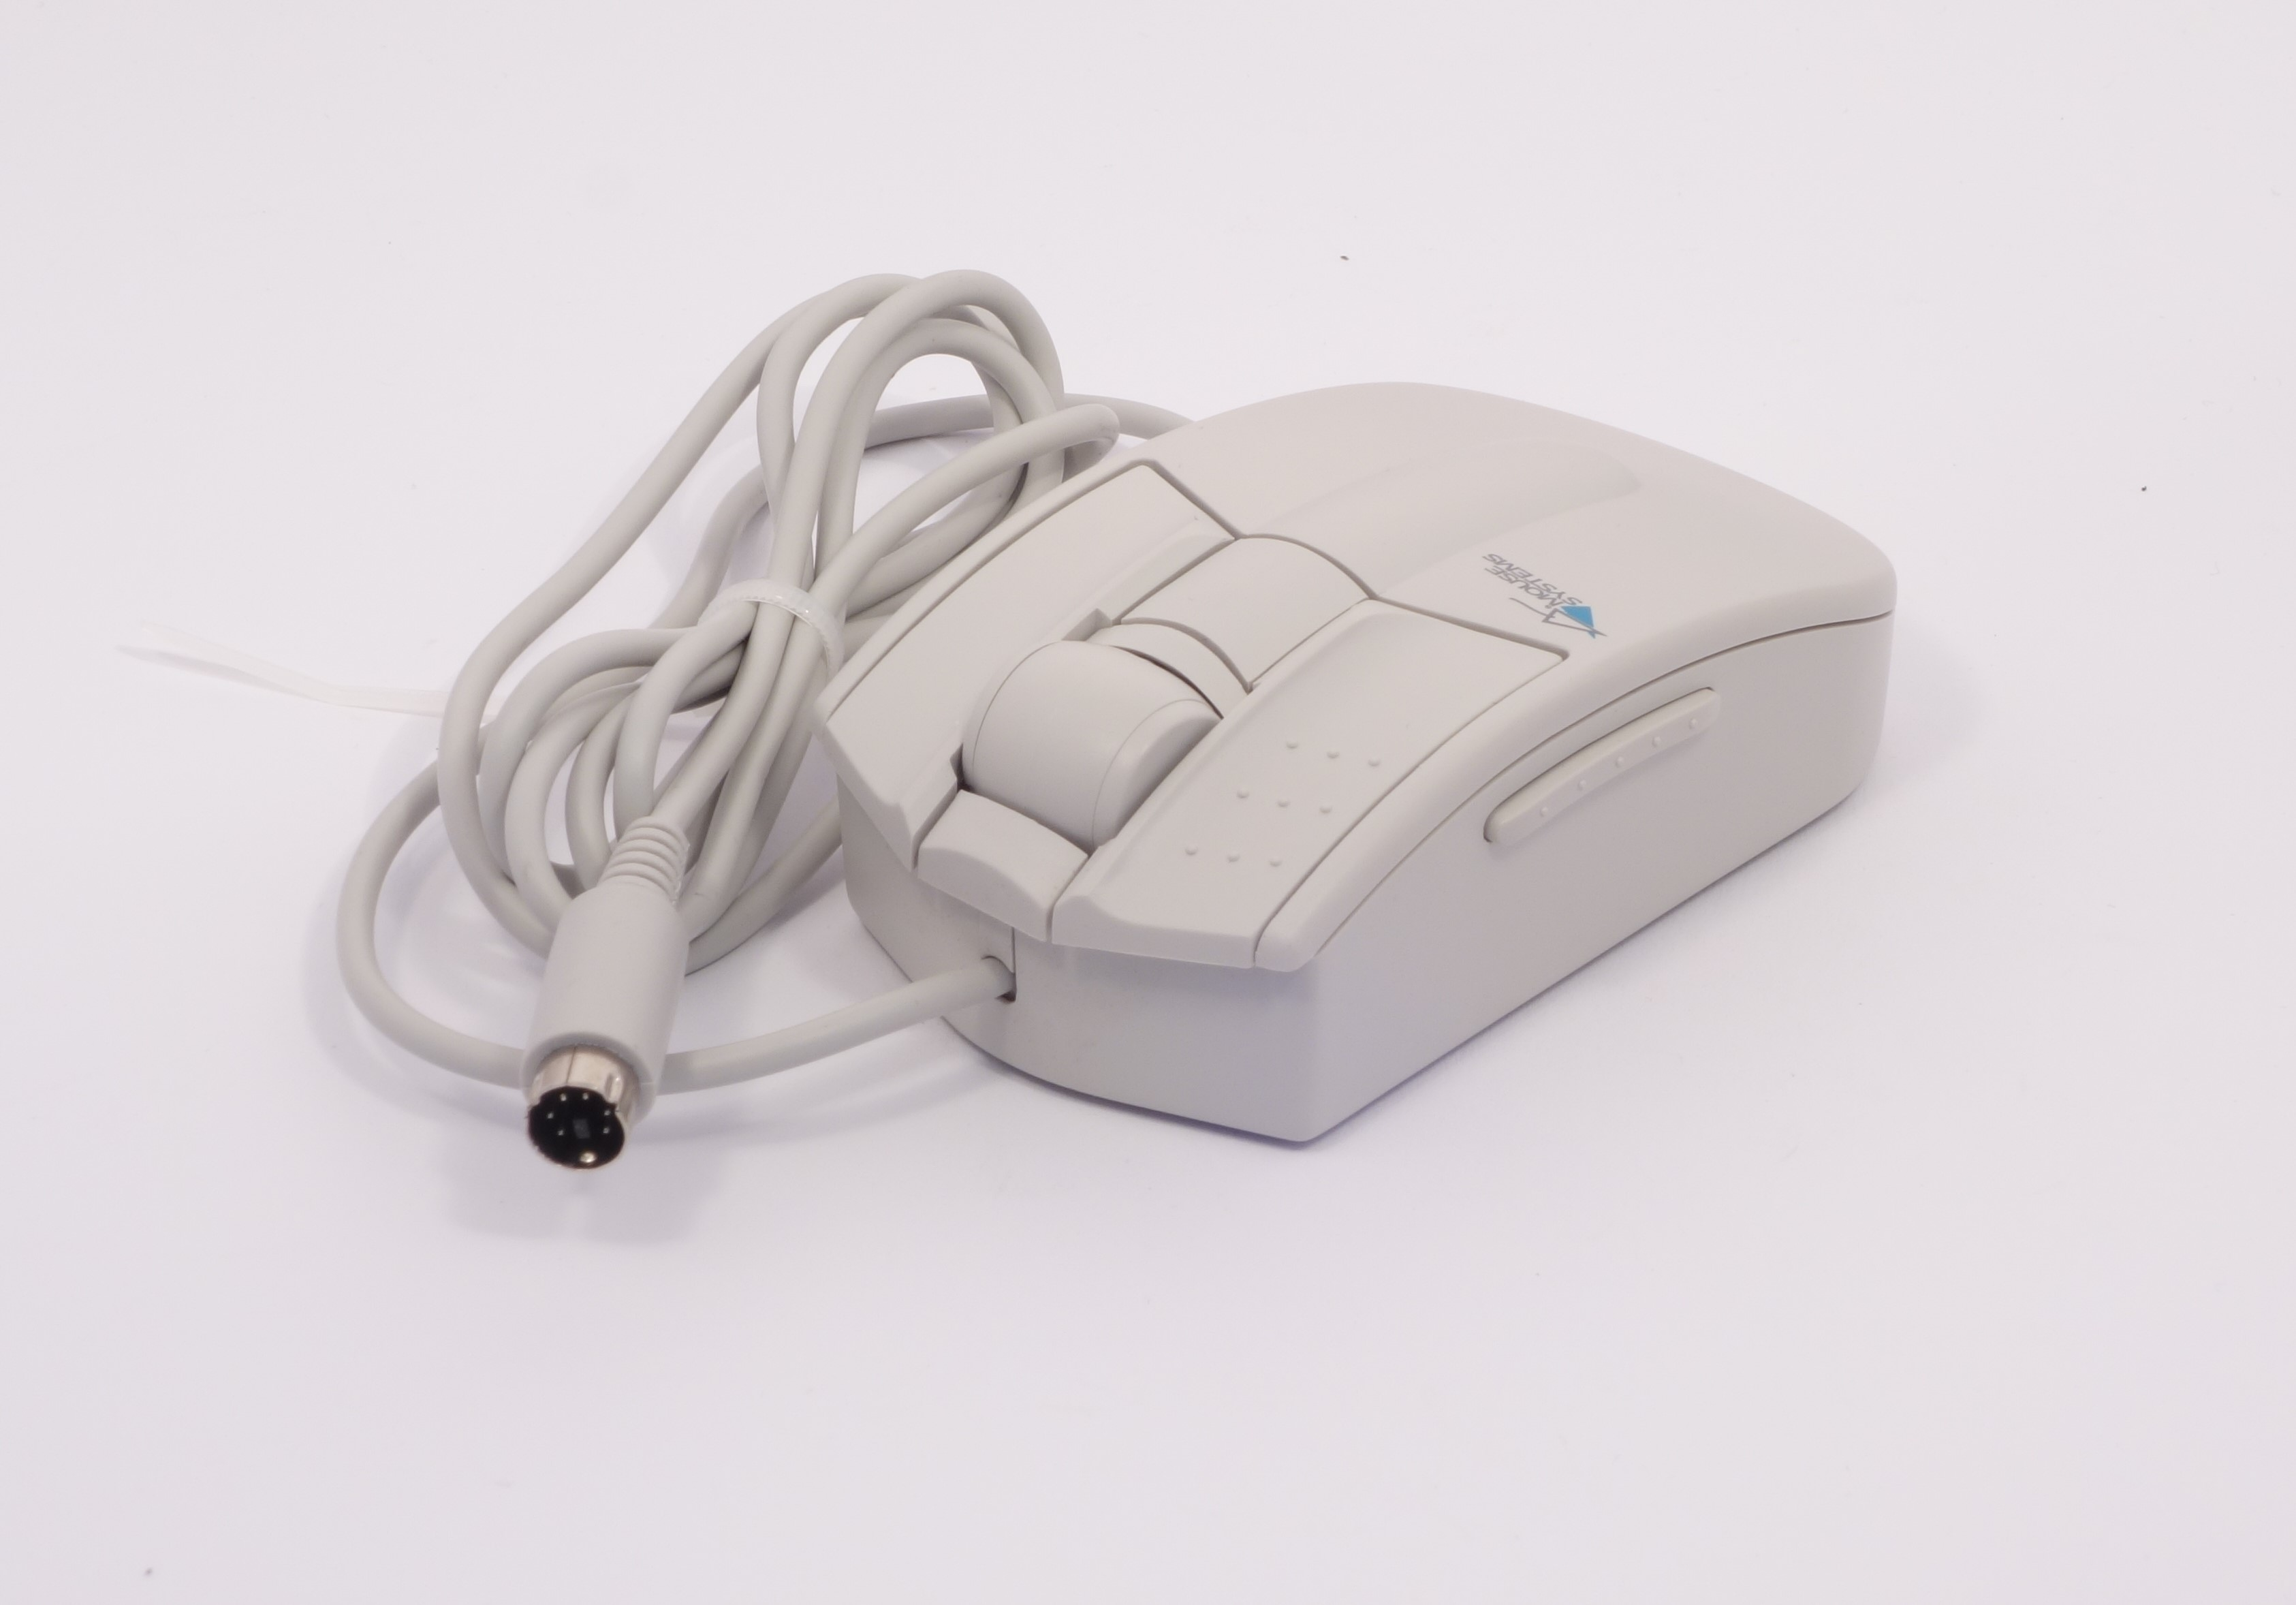
\includegraphics[scale=0.5]{1995_pro_agio_scroll_mouse/4.1.jpg}
        \label{quad-bottom}
        \caption{ProAgio Scroll Mouse}
    \end{figure}


    \begin{figure}[h]
        \centering
    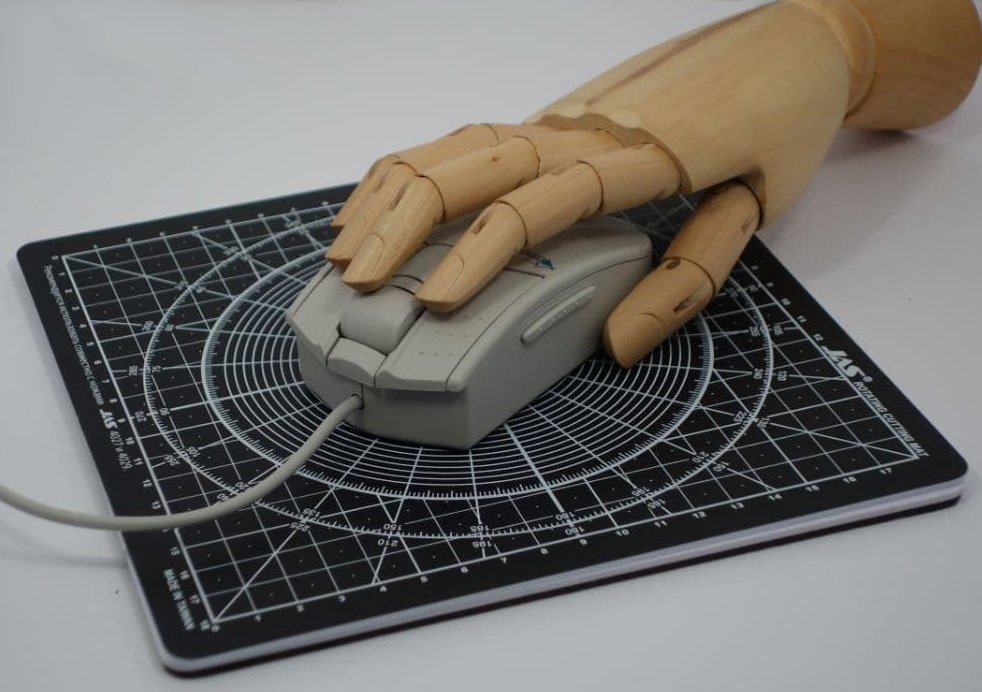
\includegraphics[scale=0.3]{1995_pro_agio_scroll_mouse/4.2.jpg}
        \label{quad-ruka}
        \caption{Изображение ProAgio Scroll Mouse с моделью руки человека}
    \end{figure}
    Стоит отметить, что идея колесика на указывающем устройстве появилась раньше, чем ProAgio Scroll Mouse, но не для прокрутки текста. Разработчики некоторых трекболов, таких как MicroSpeed  FastTRAP 1987 года, экспериментировали с вводом информации с помощью колеса, но в основном они пытались предоставить способ перемещения по координатной оси \textit{z} в программах, связанных с трехмерной графикой (в то время, как шар трекбола обеспечивал перемещение по осям \textit{x} и \textit{y}). В случае FastTRAP, фирма MicroSpeed описала колесо как «Trackwheel для указания третьей оси».
    
    Однажды разработчикам пришла идея использования «колеса оси Z» для прокрутки информации в окне.

    \begin{figure}[h]
        \centering
    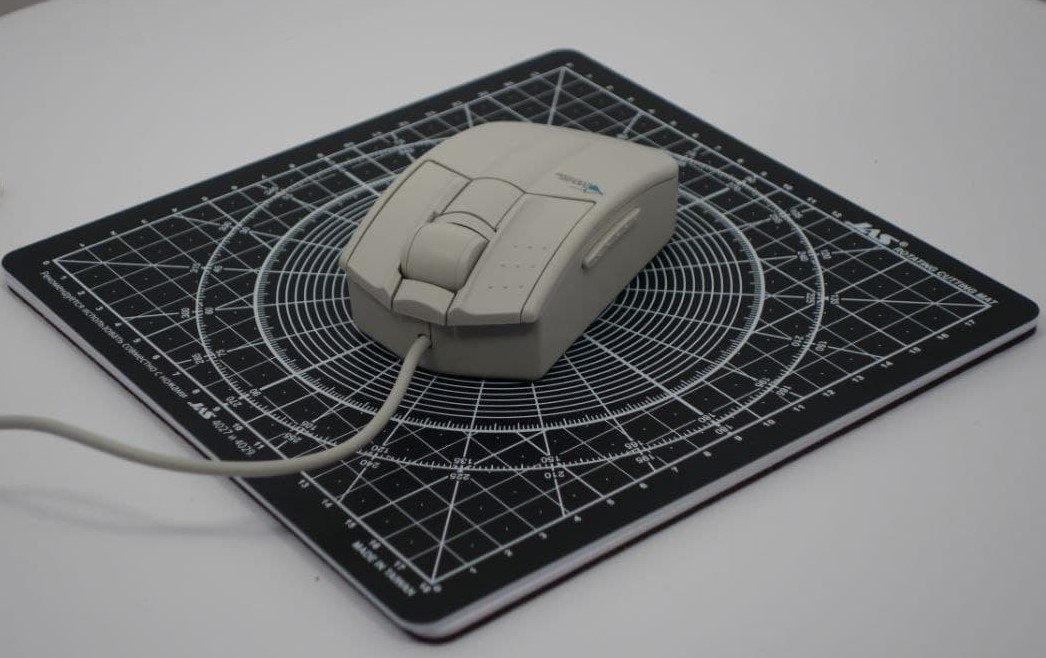
\includegraphics[scale=0.37]{1995_pro_agio_scroll_mouse/4.3.jpg}
        \label{quad-niz}
        \caption{Изображение ProAgio Scroll Mouse на размерном коврике с шагом сетки 1~см}
    \end{figure}
    
    При этом можно утверждать, что колесо прокрутки - первая настоящая инновация в конструкции мыши с момента изобретения самой мыши.

    Процитируем Эрика Мишельмана из компании Microsoft, расскрывающего особенности его появления в статье История колеса прокрутки \cite{ink}:

    «Еще в 1993 году, когда я наблюдал, как многие пользователи Excel выполняют свою работу, я заметил, что им сложно перемещать большие электронные таблицы. Поиск и переход в разные разделы часто был трудным. У меня была идея, что, возможно, поможет более продвинутое устройство ввода.
    Моей первоначальной идеей был рычаг зума. Это был просто рычаг, предположительно для вашей руки, не связанной с мышью (то есть на левой стороне клавиатуры, если вы правша). Когда вы отталкиваете ее от себя, размер таблицы уменьшается. Когда вы тянете его к себе, он снова приближается.

    Я прототипировал это, подключив джойстик к моему компьютеру и используя DDE, чтобы подключить его к Excel для масштабирования. Используя кнопку джойстика вместе с джойстиком, я также заставил его выполнять «масштабирование данных», углубляясь и выходя из контуров Excel.

    Все это показалось мне полезным, поэтому я показал это подразделению аппаратного обеспечения Microsoft. Первоначально они относились к идее, которую я представил как рычаг зума, как будто она никуда не годилась.

\newpage

    В тот момент большинство людей сочло это странным. Но сосредоточение внимания на масштабировании было очень ориентированным на Excel подходом. В частности, это был <<очень двумерный>> подход. То есть, используя приложение, которое представляет двумерные данные, такие как электронная таблица или графика, очень полезно увеличивать и уменьшать масштаб. Но основной стиль многих других приложений - это линейный поток данных, как в Word, и в таких приложениях оно не настолько полезно. Вы можете выполнять масштабирование с помощью Word, где уменьшение масштаба показывает вам многостраничный вид, а затем вы щелкаете нужную страницу и увеличиваете ее, но это не так естественно, как с электронной таблицей или графическими изображениями.
    
    Некоторые люди предложили добавить функции панорамирования и прокрутки. В частности, я помню, как Крис Грэм сказал, что масштабирование слишком ограничивает, и его также следует панорамировать. В ответ на эти отзывы я добавил панорамирование к прототипу, поэтому, перемещая джойстик из стороны в сторону и вперед-назад, Excel прокручивал таблицу в соответствующем направлении.

    Примерно в это время специалисты по аппаратному обеспечению включились в обсуждение и сообщили, что они рассматривали возможность добавления колесика к мыши, но не знали, для чего оно будет использоваться. Навигация по документам отвечала на этот вопрос, поэтому они сказали, что если бы я мог заставить Office поддерживать эту функцию, они бы ее реализовали. На самом деле речь шла о поддержке в приложениях Excel и Word, поскольку они были «гориллами весом 800 фунтов» - если Excel и Word что-то поддерживали, то другие приложения Office следовали за ними, а если Office в целом что-то поддерживает, то все остальные тоже идут следом (это было начало 1993 года, когда Office был основной причиной использования компьютеров большинством людей)».

\begin{figure}[h]
        \centering
    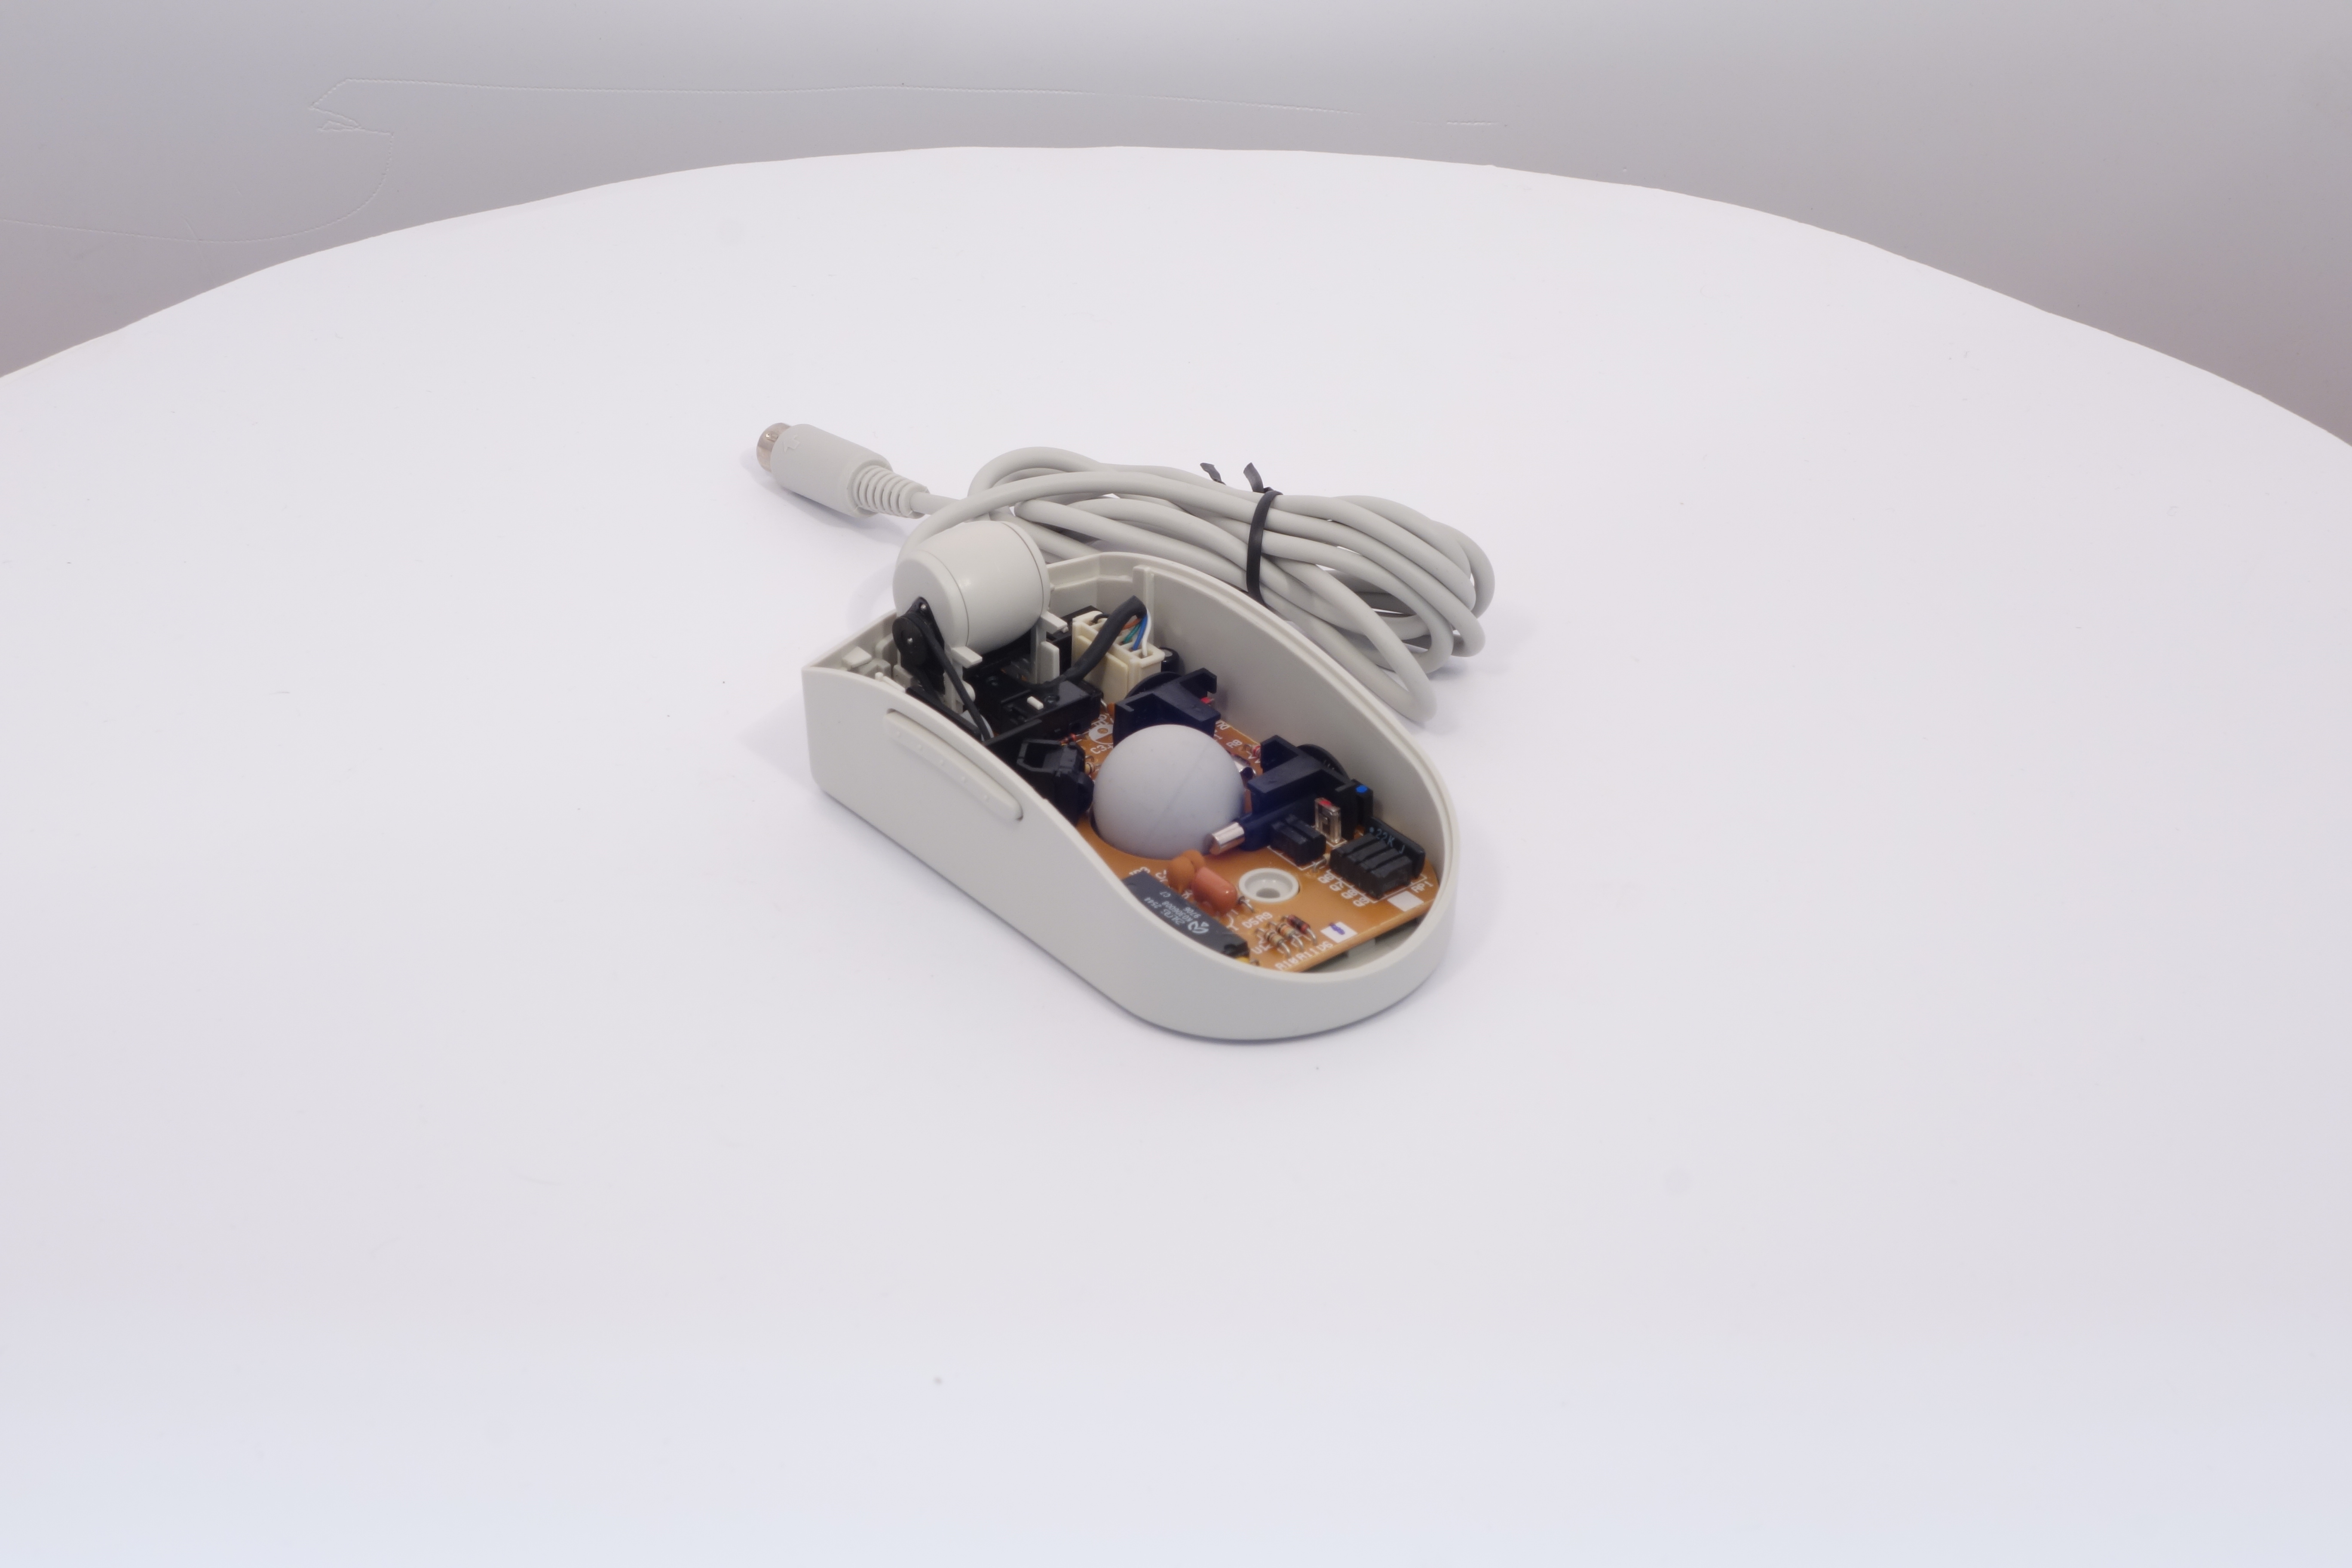
\includegraphics[scale=0.4]{1995_pro_agio_scroll_mouse/6.3.jpg}
        \label{quad-kov}
        \caption{Изображение ProAgio Scroll Mouse в разобранном виде}
    \end{figure}

   Изображение ProAgio Scroll Mouse в разобранном виде показано на рисунке 2.16. Как можно видеть, Мышь использует оптико-механическую технологию (разрешение составляет 400 точек на дюйм). Также среди особенностей следует отметить, что для передачи вращения колеса разработчики использовали ременную передачу с помощью резинового пасика, что никогда не встречается в современных устройствах.
\begin{thebibliography}{9}
\bibitem {ink} CODING HORROR \url{https://blog.codinghorror.com/meet-the-inventor-of-the-mouse-wheel/}
\bibitem {yt} oldmouse.com \url{https://www.oldmouse.com/mouse/mousesystems/scroll.shtml}
\end{thebibliography}
\end{document}
